\documentclass[../TDE4-E5.tex]{subfiles}%

\begin{document}
\section[s]"1"{RLC sur $q$ et bilan d'énergie}

\enonce{%
	\noindent

	\begin{minipage}{0.7\linewidth}
		Un circuit électrique est composé d'une résistance $R$, d'une bobine
		d'inductance $L$ et d'un condensateur de capacité $C$. Ces dipôles sont
		disposés en série et on soumet le circuit à un échelon de tension tel que~:
		$ \left\{
			\begin{array}{rcl}
				e(t<0)    & = & 0 \\
				e(t\geq0) & = & E
			\end{array}
			\right.$.
		On pose $\gamma = \dfrac{R}{2L}$ et $\w_0 = \dfrac{1}{\sqrt{LC}}$
	\end{minipage}
	\begin{minipage}{0.3\linewidth}
		\centering
		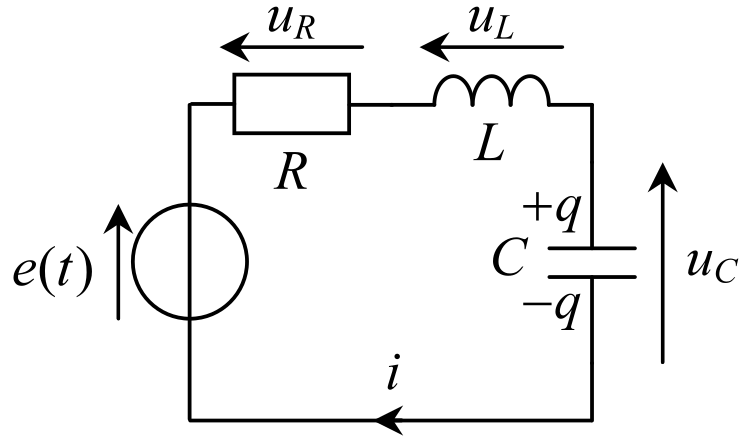
\includegraphics[width=\linewidth]{rlc_energie}
	\end{minipage}
}%

\QR{%
	Expliquer simplement pourquoi à $t = 0^-$ la charge $q$ et le courant
	$i$ sont nuls.
}{%
	À $t=0^-$, le circuit est depuis longtemps sous la tension $e=0$~; il a donc
	atteint son régime permanent, et le condensateur s'est déchargé et est
	équivalent à un interrupteur ouvert~: forcément,
	\begin{equation*}
		\boxed{i(0^-) = 0} \qet \boxed{q(0^-) = Cu(0^-) = 0}
	\end{equation*}
}%

\QR{%
	Montrer que l'équation différentielle vérifiée par la charge $q(t)$ du
	condensateur pour $t > 0$ est~:
	\[ \dv[2]{q}{t} + 2\gamma \dv{q}{t} + \w_0{}^2 q = \frac{E}{L}\]
	Préciser, en les justifiant, les valeurs initiales de la
	charge $q(0^+)$ et de sa dérivée.
}{%
	Avec une loi des mailles, les RCT de la résistance, de la bobine et du
	condensateur et la relation $i = \dv{q}{t}$, on a
	\begin{gather*}
		u_L + u_R + u_C = E
		\Leftrightarrow
		L \dv{i}{t} + Ri + \frac{q}{C} = E\\
		\Leftrightarrow
		L \dv[2]{q}{t} + R \dv{q}{t} + \frac{q}{C} = E
		\Leftrightarrow
		\dv[2]{q}{t} + 2\gamma \dv{q}{t} + \frac{q}{C} = \frac{E}{L}
	\end{gather*}
	Concernant les conditions initiales, la tension aux bornes d'un condensateur
	est continue donc sa charge aussi, c'est-à-dire
	\[\boxed{q(0^-) = q(0^+) = 0}\]
	et comme le courant traversant une bobine est également continu, on a
	\[i(0^-) = i(0^+) = 0\qsoit \boxed{ \qty(\dv{q}{t})_{0^+} = 0}\]
}%

Le circuit présente différents régimes suivant les valeurs de $R$, $L$ et $C$.
On suppose dans la suite la condition $\w_0 > \gamma$ réalisée.

\QR{%
Montrer que l'expression de la charge pour $t > 0$ peut se mettre sous la
forme
\[q(t) = [A \cos(\w t) + B \sin(\w t)] \exr^{-\gamma t} + D\]
avec $A$, $B$ et $D$ des constantes à exprimer en fonction de $C$, $E$,
$\w_0$ et $\gamma$.
}{%
L'équation caractéristique de discriminant $\Delta$ de l'équation homogène
est
\[r^2 + 2\gamma r + \w_0{}^2 = 0 \Rightarrow \Delta = 4(\gamma^2
	-\w_0{}^2)\]
Comme $\w_0 > \gamma$, on a $\Delta <0$ et on est donc dans un régime
pseudo-périodique. On aura donc
\begin{gather*}
	r_\pm = -\frac{\cancel{2}\gamma}{\cancel{2}} \pm \Ir
	\frac{1}{\bcancel{2}}\sqrt{\bcancel{4}(\w_0{}^2 - \gamma^2)}
	\Leftrightarrow
	\boxed{r_\pm = -\gamma \pm \Ir \w}
	\qavec
	\boxed{\w = \sqrt{\w_0{}^2 - \gamma^2}}
\end{gather*}
La solution particulière est $\frac{E}{L\w_0{}^2} = CE$, donc on aura la forme
générale
\begin{equation*}
	\boxed{q(t) = \exr^{-\gamma t} \left( A\cos\wt + B\sin\wt \right) +
		CE}
\end{equation*}
Avec la première CI,
\[q(0) = A+CE = 0 \Leftrightarrow \boxed{A = -CE}\]
et avec la seconde,
\[\qty(\dv{q}{t})_0 = -\gamma A + B\w = 0
	\Leftrightarrow
	\boxed{B = -CE \frac{\g}{\sqrt{\w_0{}^2 - \g^2}}}\]
soit finalement
\begin{equation*}
	\boxed{q(t) = CE -
		CE \exr^{-\gamma t}
		\left( \cos\wt +
		\frac{\g}{\sqrt{\w_0{}^2 - \g^2}}\sin\wt
		\right)}
\end{equation*}
}%

\QR{%
	Exprimer le courant $i(t)$ dans le circuit pour $t > 0$ en fonction de
	$C$, $E$, $\w_0$ et $\gamma$.
}{%
	On dérive $q$~:
	\begin{equation*}
		\boxed{i(t) = CE \frac{\w_0{}^2}{\w}\exr^{-\g t}\sin\wt}
	\end{equation*}
}%

\QR{%Donner l'allure des courbes $q(t)$ et $i(t)$. Quelles sont leurs valeurs à
	la fin du régime transitoire~? Justifier par des considérations simples ces
	valeurs atteintes.
}{%
	La charge finale atteinte est $CE$ et le courant final est nul. Ces valeurs
	se retrouvent facilement en remarquant qu'en régime permanent, le
	condensateur se comporte comme un interrupteur ouvert et la bobine comme un
	fil~; le courant est alors nul, et ainsi les tensions aux bornes de $L$ et
	$R$ le sont également~: la tension $E$ du circuit est entièrement dans
	$u_C$, et sa charge est donc $CE$.
	\begin{center}
		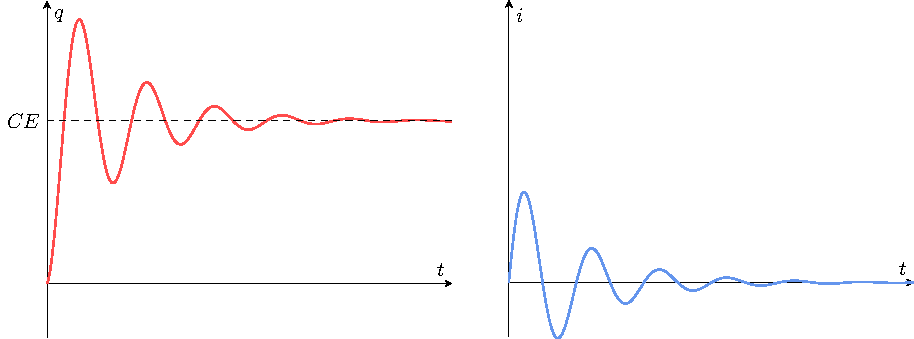
\includegraphics[width=\linewidth]{energ_amorti-qi}
	\end{center}
}%

\QR{%
	Déterminer l'énergie totale $\Ec_G$ fournie par le générateur ainsi que
	l'énergie $\Ec_{LC}$ emmagasinée dans la bobine et le condensateur à la fin
	du régime transitoire en fonction de $C$ et $E$. En déduire l'énergie
	dissipée par effet \textsc{Joule} dans la résistance. Ces résultats
	dépendent-ils du régime particulier dans lequel se trouve le circuit~?
	Interpréter le résultat paradoxal qui apparaît dans le cas limite $R
		\longrightarrow 0$.
}{%
	Un bilan de puissance sur le circuit, (i.e.\ \textbf{loi des mailles$\times
			i$}) donne
	\[ \Pc_L + \Pc_C + \Pc_J = \Pc_G \Rightarrow \boxed{\Ec_{LC} + \Ec_J = \Ec_G}\]
	On trouve donc naturellement que l'énergie du générateur se répartit entre
	la bobine, l'inductance et la résistance. On va donc déterminer $\Ec_G$ et
	$\Ec_{LC}$ pour trouver $\Ec_J$ par différence.\bigbreak
	L'énergie fournie par le générateur s'obtient en intégrant la puissance
	fournie $Ei$ par le générateur entre $t=0$ et $t \rightarrow \infty$. En se
	rappelant que $i = \dv{q}{t}$, cette intégrale se ramène à une simple
	intégration sur $q$ de valeur initiale 0 et de valeur finale $CE$~:
	\[ \Ec_G = \int_{0}^{\infty} Ei \dt = \int_{0}^{CE} E\dd q = E \left[
			q \right]^{q=0}_{q=CE} \Leftrightarrow \boxed{\Ec_G = CE^2}\]
	L'énergie $\Ec_{LC}$ emmagasinée par l'inductance et la capacité se calcule
	par différence des énergies stockées dans ces dipôles entre l'instant final
	et l'instant initial. Or, les deux dipôles sont initialement déchargés, et
	comme $i = 0$ à la fin l'énergie de la bobine est nulle. Ainsi,
	\[\Ec_{LC} = \left[ \frac{1}{2}Li(t)^2 + \frac{1}{2} \frac{q(t)^2}{C}
			\right]_{t=0}^{t=\infty} \Leftrightarrow \boxed{\Ec_{LC} = \frac{1}{2}CE^2}\]
	Ainsi,
	\[ \Ec_{J} = \Ec_G - \Ec_{LC} \Leftrightarrow \boxed{\Ec_J =
			\frac{1}{2}CE^2}\]
	Ces calculs sont indépendants du régime dans lequel se trouve le circuit.
	L'énergie fournie par le générateur est deux fois plus grande que celle
	stockée par la bobine et le condensateur, \textbf{indépendamment de la
		valeur de la résistance du circuit}.\smallbreak
	Extrapolé à $R \longrightarrow 0$, ce résultat semble contredire le
	principe de conservation de l'énergie, puisque la seconde moitié d'énergie
	ne peut plus être dissipée par effet \textsc{Joule}. En fait, pour $R
		\longrightarrow 0$, le circuit oscille de façon sinusoïdale~: on n'atteint
	jamais de régime permanent continu, et la bobine et le condensateur stockent
	et restituent alternativement de l'énergie.
}%

\end{document}
